% ICML 2026 Preprint -- Work in Progress
% Last updated: December 2025
%
% Build with: make paper (from project root)
% See paper/WORKFLOW.md for AI agent instructions

\documentclass{article}

% Recommended packages
\usepackage{microtype}
\usepackage{graphicx}
\usepackage{subcaption}
\usepackage{booktabs}
\usepackage{hyperref}
\usepackage{amsmath,amssymb,mathtools,amsthm}
\usepackage[capitalize,noabbrev]{cleveref}
\usepackage{algorithm}
\usepackage{algorithmic}

% ICML 2026 style (preprint mode)
\usepackage[preprint]{icml2026}

% Path to figures (relative to paper/ directory, set via TEXINPUTS)
\graphicspath{{../figures/}}

%%%%%%%%%%%%%%%%%%%%%%%%%%%%%%%%
% THEOREMS AND MACROS
%%%%%%%%%%%%%%%%%%%%%%%%%%%%%%%%

\theoremstyle{plain}
\newtheorem{theorem}{Theorem}[section]
\newtheorem{proposition}[theorem]{Proposition}
\newtheorem{lemma}[theorem]{Lemma}
\newtheorem{corollary}[theorem]{Corollary}
\theoremstyle{definition}
\newtheorem{definition}[theorem]{Definition}
\newtheorem{assumption}[theorem]{Assumption}
\theoremstyle{remark}
\newtheorem{remark}[theorem]{Remark}

\newcommand{\E}{\mathbb{E}}
\newcommand{\Q}{\hat{Q}}

\icmltitlerunning{Inference-Time Guidance for Diffusion Policies}

\begin{document}

\twocolumn[
\icmltitle{Inference-Time Guidance for Diffusion Policies\\in Online Reinforcement Learning\\[0.5em]\normalsize\textit{Preprint -- Work in Progress}}

\begin{icmlauthorlist}
  \icmlauthor{Philip Nielsen}{harv}
\end{icmlauthorlist}

\icmlaffiliation{harv}{School of Engineering and Applied Sciences, Harvard University}
\icmlcorrespondingauthor{Philip Nielsen}{pnielsen@seas.harvard.edu}

\icmlkeywords{Reinforcement Learning, Diffusion Policies, Training-Free Guidance, Model-Based RL, Compositional AI}

\vskip 0.3in
]

\printAffiliationsAndNotice{}

\begin{abstract}
Diffusion policies are an expressive policy class for continuous-control reinforcement learning, but current online methods such as DPMD couple the critic tightly to training by reweighting the denoising loss with exponentiated $Q$-values.
We explore an alternative: fit a diffusion policy with simple behavior cloning, then apply $Q$-based guidance or filtering only at inference time.
On MuJoCo HalfCheetah-v4, we find that a many-particle Boltzmann selection baseline (no $Q$-reweighting at training time) matches the performance of the DPMD baseline while using constant learning rates suitable for continual learning.
We also implement MALA-corrected $Q$-guidance that samples from the mirror-descent target policy using a single action particle, and model-based variants that replace $Q$ with a compositional objective built from learned dynamics, reward, and value networks.
As of yet, the simpler inference-time methods currently outperform the model-based ones, but all configurations train stably online from scratch---a proof of concept for more compositional approaches to diffusion-policy RL.
\end{abstract}

\section{Introduction}
\label{sec:intro}

Deep reinforcement learning has achieved impressive results in continuous control, yet standard Gaussian policies struggle to represent multi-modal action distributions and have no mechanism for scaling computation at inference time.
Diffusion models \citep{ho2020denoising,song2021sde} offer an appealing alternative: by learning to reverse a gradual noising process, they provide expressive policies with simple denoising score-matching losses. Using guidance, they can be flexibly repurposed for different objectives without retraining. Guidance signal can come from predictions of future states and rewards given partially denoised actions, allowing for planning at inference time as well.
Recent work has adapted diffusion models to policy learning in both offline and online RL \citep{janner2022diffuser,wang2023diffusion,ma2025soft}.

In mirror descent, the target update is 
\begin{equation}
  \pi(a\mid s) \propto \pi_\mathrm{old}(a\mid s) \exp\{\lambda Q(s,a)\}.
  \label{eq:md-tilt}
\end{equation}
Diffusion policies are typically trained with samples from the target distribution, which are not available in the online RL setting.
The Diffusion Policy Mirror Descent (DPMD) framework \citep{ma2025soft} approximately implements this update by using $Q$ to select the best among many sampled actions at inference time, then behavior-cloning the replay buffer of its own sampled actions, reweighting by a factor of $\exp\{\lambda Q(s,a)\}$.

While effective and efficient, we note a number of ways our methods attempt to improve upon it.
First, the method relies on multiple departures from pure mirror descent in order for it to work: mainly the injection of noise in action choices and the practice of sampling the best of many action particles at inference time.
Second, implementing the update rule at training time by reweighting reduces the effective sample size compared to pure behavior cloning, potentially reducing the information learned from each transition. 
Third, the method makes no use of gradients of the critic. Better actions are only discovered if they are sampled by the base policy and up-weighted at training time. By contrast, inference time guidance uses gradients to direct samples toward high-reward regions. This is expected to scale better as the dimension of the action space increases.
Fourth, it makes no use of world models. Some of our proposed methods estimate $Q$ as a composition of world and value models, making it more likely to generalize farther out of distribution at inference time and providing a better reason to scale up compute. 

\paragraph{A progression of inference-time methods.}
We explore a complementary, more compositional perspective by asking: \emph{Can we train diffusion policies with simpler, more stable objectives, and move most of the mirror-descent structure and planning to inference time?}
We investigate a progression of methods, each adding a layer of modeling complexity to the previous:
\begin{enumerate}
  \item \textbf{Constant-weight diffusion + Boltzmann selection.} Target the mirror-descent update distribution by sampling many actions from the base policy and selecting an action to step the environment with probability proportional to $\exp\{\lambda Q(s,a)\}$. Distill the tilted action distribution into the base policy by behavior cloning the replay buffer (uniform weights).
  \item \textbf{Inference-time $Q$-guidance with MALA.} Directly sampling the mirror-descent policy using training-free guidance. Combined with MCMC (MALA) at each noise level, this ensures that the distribution of sampled actions at each noise level matches that of the energy function given by the TFG objective and smoothly converges to the target policy at zero noise.
  \item \textbf{Model-based compositional guidance.} Estimate $Q$ by one-step decomposition $Q(s,a) = \E[r(s,a,s') + \gamma V(s')]$ built from separately learned dynamics, reward, and value networks. Dynamics models can be either deterministic or probabilistic (diffusion) models.
  \item \textbf{Short-horizon planning.} Extend the model-based setup by planning over short action sequences. As the planning horizon gets longer, the compositional objective is comprised more of stationary targets (reward and dynamics) which depend only on the environment and are learned by supervised learning on the replay buffer, and less of non-stationary targets (value) which depend on and lag behind the policy during learning. 
\end{enumerate}
The ideal outcome of this research direction is that each additional layer of complexity should improve performance over the previous one, allowing users to find the ideal allocation of compute at training and inference time, which has been demonstrated to be a consequential consideration in settings such as language and games.
In our current experiments, this goal is not yet achieved: the simpler inference-time methods outperform the more complex model-based variants. However, we demonstrate that each configuration can be trained stably from scratch in an online RL setting, which we believe is an important proof of concept and promising sign for future work. In addition, two methods come close to the performance of the DPMD baseline.

\section{Related Work}
\label{sec:related}

We organize our discussion of related work around the key components of our approach: diffusion models and guidance mechanisms, diffusion policies for RL, inference-time action selection, and model-based compositional planning.

\paragraph{Diffusion models and guidance.}
Denoising diffusion probabilistic models (DDPMs) \citep{ho2020denoising} and score-based SDE models \citep{song2021sde} learn to reverse a gradually noised forward process.
Classifier guidance \citep{dhariwal2021beatgans} and classifier-free guidance \citep{ho2022classifierfree} modify the sampling dynamics by adding gradients of external or internal classifiers.
Training-free guidance (TFG) frameworks \citep{ye2024tfg,bansal2023universal} generalize this idea to arbitrary objectives evaluated on Tweedie-style clean estimates and highlight the need for careful treatment of guidance strength and off-manifold drift.
Energy-based diffusion with MCMC corrections \citep{du2023reduce_reuse_recycle} shows how to combine energy terms with the base diffusion model while correcting the sampler via Metropolis--Hastings steps.
These techniques have been applied primarily in computer vision; we adapt them to continuous-control RL.

\paragraph{Diffusion policies for reinforcement learning.}
In \emph{offline} RL, Diffuser \citep{janner2022diffuser} applies trajectory-level diffusion by diffusing entire state-action trajectories and conditioning on desired outcomes at inference time.
\citet{wang2023diffusion} study diffusion policies as an expressive policy class for offline continuous control, and subsequent work has explored diffusion for imitation learning and goal-conditioned control \citep{chi2023diffusion,reuss2023goal}.

In \emph{online} RL, DPMD and SDAC \citep{ma2025soft} use diffusion policies with $Q$-weighted training losses derived from a mirror-descent interpretation.
DPMD implements the tilted policy in \cref{eq:md-tilt} by reweighting the denoising loss according to exponentiated $Q$-values and selecting among a small set of denoised candidates at decision time.
Our work builds directly on DPMD but takes a different approach: we \emph{remove} $Q$ from the training loss entirely and push all mirror-descent structure to inference time.

\paragraph{Inference-time action selection and Boltzmann policies.}
The idea of sampling actions proportionally to exponentiated $Q$-values has a long history in maximum-entropy RL.
Soft Q-learning \citep{haarnoja2017sql} and Soft Actor-Critic \citep{haarnoja2018sac} learn Boltzmann policies $\pi(a|s) \propto \exp(Q(s,a)/\tau)$ by optimizing an entropy-regularized objective.
Recent work on diffusion Q-sampling \citep{lu2024diffusionql} uses diffusion models to sample from such Boltzmann distributions in continuous action spaces.
DPMD's batch action sampling trick---generating multiple candidates and selecting based on $Q$---is a practical instantiation of this idea, though with argmax rather than stochastic selection.

Our constant-weight baseline takes this further by \emph{completely separating} the roles of training and selection: the diffusion policy is trained purely by behavior cloning with uniform weights, and all $Q$-dependent selection happens at inference time via many-particle Boltzmann sampling.
This clean separation reveals the \emph{constant-weight anomaly}: in our setting, most of the performance benefit attributed to $Q$-reweighted training actually comes from inference-time selection.

\paragraph{Model-based RL and compositional planning.}
Model-based RL has a long history \citep{sutton1990dyna}, with recent successes in latent world models \citep{hafner2020dreamer,hafner2023dreamerv3} and planning with learned dynamics \citep{schrittwieser2020muzero}.
These approaches typically use non-diffusion policy classes (e.g., Gaussian or discrete).
\citet{ajay2023conditional} argue that conditional generative models can serve as composable decision-makers across tasks.
Diffuser \citep{janner2022diffuser} can be viewed as model-based planning in trajectory space, but it targets offline RL and does not separately learn dynamics, reward, and value components.

Our model-based variants adopt a modular structure: we train separate dynamics, reward, and value networks, combine them into the compositional objective $\Q(s,a) = \E[r+\gamma V]$, and use this to guide a diffusion policy at inference time.
To our knowledge, this is the first system to independently train all four components (diffusion policy, dynamics model, reward model, value function) online from scratch and use their composition for inference-time guidance.

\paragraph{Diffusion-based dynamics models.}
Several works have explored diffusion models for learning transition dynamics.
\citet{rigter2023worldmodels} use diffusion dynamics for trajectory generation consistent with online policies.
DiWA \citep{diwa2025} combines diffusion policies with world models for offline adaptation.
Our diffusion dynamics variant goes further by \emph{jointly} training the diffusion policy and diffusion dynamics model online, using them in a nested planner that refreshes next-state particles during action sampling.
Although our current results show that this additional complexity does not yet improve over simpler methods, we demonstrate that stable online training of such a multi-diffusion system is achievable.

\section{Background}
\label{sec:background}

We briefly summarize the base DPMD setup and training-free guidance from a mathematical perspective.

\subsection{Diffusion policies and DPMD}

We parameterize the policy as a conditional diffusion model $\pi_\theta(a\mid s)$ together with twin Q-functions $Q_1,Q_2$.
A fixed forward process progressively adds Gaussian noise to a clean action $a_0$ to obtain $a_T$, and a reverse process learns to denoise $a_T$ back to $a_0$ via denoising score matching.

DPMD implements a mirror-descent-style policy update by combining off-policy TD learning for $Q_1,Q_2$ with a \emph{weighted} denoising loss for the policy.
The diffusion loss takes the form
\begin{equation}
  \mathcal{L}_{\text{diff}} = \E\big[ w(s,a) \; \| \epsilon_\theta(a_t,s,t) - \epsilon \|^2 \big],
\end{equation}
where $a$ is the clean replay action and $w(s,a)$ is derived from a standardized version of $Q_{\min}(s,a) = \min(Q_1,Q_2)$.
In the original implementation the running mean $m$ and standard deviation $\sigma$ of $Q_{\min}$ are tracked and scores are clipped, exponentiated, and renormalized to keep the \emph{effective sample size} of the weights close to the batch size.
An earlier bug normalized as $Q_{\min} - m/\sigma$ instead of $(Q_{\min}-m)/\sigma$; on HalfCheetah-v4 we find that correcting this bug \emph{reduces} performance (from about $11268$ to about $10263$ average return), suggesting that the original normalization acted as an accidental but well-tuned temperature.

At inference time, DPMD draws $N$ action candidates from the policy and selects the argmax under $Q_{\min}$.

\subsection{Training-free guidance and Tweedie estimates}

Training-free guidance (TFG) \citep{ye2024tfg,bansal2023universal} views guidance as composing an energy term $\lambda J(s,a)$ with the base diffusion model and adjusting the reverse process accordingly.
Given a noisy action $a_t$ and a learned noise predictor $\epsilon_\theta(a_t,s,t)$, Tweedie's formula provides an estimate of the clean action
\begin{equation}
  \hat{a}_0 = \frac{a_t - \sqrt{1-\bar{\alpha}_t}\, \epsilon_\theta(a_t,s,t)}{\sqrt{\bar{\alpha}_t}},
\end{equation}
where $\bar{\alpha}_t$ is the cumulative product of $(1-\beta_t)$ along the noise schedule.
A simple TFG update modifies the noise prediction as
\begin{equation}
  \epsilon_{\text{guided}} = \epsilon_\theta - \lambda \sigma_t \nabla_{a_t} J(s,\hat{a}_0(a_t)),
\end{equation}
which heuristically moves samples toward decreasing energy $J$.
However, this modification alone does not guarantee sampling from the correctly tilted distribution.

\section{Methods}
\label{sec:methods}

We now describe the main algorithmic families explored in this work, organized in order of increasing modeling complexity.
Each method represents a different point on a spectrum from pure inference-time filtering (Boltzmann selection) through inference-time gradient-based guidance (MALA) to full model-based compositional planning.
We begin with the simplest approach and progressively add components.

\subsection{Constant-weight diffusion and many-particle Boltzmann selection}
\label{sec:boltzmann}

The simplest variant in our progression dispenses with training-time weighting entirely and treats the diffusion policy as a pure behavior-cloning model trained with uniform weights on replay actions.
At inference time, we draw $N$ denoised candidates $a^{(1)},\dots,a^{(N)}$ from the policy and perform \emph{Boltzmann selection}: we sample an action index $I$ from a categorical distribution with probabilities proportional to exponentiated Q-values,
\begin{equation}
  P(I = i) \propto \exp\{\lambda_{\text{sel}} Q(s,a^{(i)})\}.
\end{equation}
The executed action is then $a^*(s) = a^{(I)}$.
This is \emph{not} deterministic best-of-$N$ selection (which would correspond to $\lambda_{\text{sel}} \to \infty$), but rather a stochastic procedure that preferentially selects high-Q actions while maintaining exploration.

Our best configuration uses $N=128$ particles and a selection temperature $\lambda_{\text{sel}}=64$, achieving $10866$ average return (SE $\approx 370$) over five seeds.
This variant does not use $Q$ in the diffusion loss and consults it only through the selection distribution at decision time.

\subsection{Inference-time $Q$-guidance with MALA}
\label{sec:mala}

The next level of complexity adds gradient-based guidance at inference time.
Rather than simply filtering among candidates, we actively steer the diffusion sampling process toward high-$Q$ regions using the critic's gradient.

We consider an energy-based parameterization of the diffusion policy and add a small number of MALA correction steps at each diffusion level.
In energy mode, the policy outputs a scalar energy $E_\theta(a_t,s,t)$ and the score used in the diffusion loss is $\nabla_{a_t} E_\theta$.

We then define, at each level $t$, a total energy that composes the diffusion energy with the critic:
\begin{equation}
  E_t(a_t,s) = E_\theta(a_t,s,t) - \lambda_t Q_{\text{agg}}(s,a_0(a_t)),
\end{equation}
where $a_0(a_t)$ is the Tweedie-style clean estimate and $Q_{\text{agg}}$ is either $Q_{\min}$ or the mean of $Q_1,Q_2$.
The guidance strengths $\lambda_t$ are derived from a schedule type.

At each diffusion level, the sampler alternates a few MALA steps with standard reverse-diffusion prediction steps.
A single MALA step proposes
\begin{equation}
  a_t' = a_t - \eta \nabla_{a_t} E_t(a_t,s) + \sqrt{2\eta}\, z,
\end{equation}
with $z\sim \mathcal{N}(0,I)$, followed by a Metropolis--Hastings accept/reject step.
The step size $\eta$ is adapted to target an acceptance rate near $0.574$ \citep{RobertsTweedie1996MALA}.

In our best-performing configuration on HalfCheetah-v4 we disable $Q$-based reweighting at training time, use a single action particle, and apply a modest amount of MALA correction per diffusion level so that the critic is consulted only at sampling time.

\paragraph{Relation to prior work.}
Training-free guidance and MCMC corrections have been studied extensively for generative diffusion models in computer vision \citep{ye2024tfg,du2023reduce_reuse_recycle}.
Online diffusion policies have been explored via reweighted score matching \citep{ma2025soft}, and energy-based RL methods have used Langevin dynamics for policy sampling \citep{haarnoja2017sql}.
To our knowledge, our MALA-guided configuration is the first to \emph{jointly}: (i) train a diffusion policy for continuous-control RL from scratch with constant-weight behavior cloning, and (ii) apply per-diffusion-level MALA corrections on a combined diffusion+$Q$ energy at inference time.
This differs from DPMD in that the critic is used only for sampling rather than in the training loss. Compared to training-free gradient-guidance methods such as TFG, which bias the reverse dynamics without MH correction, we follow Du et al. \citep{du2023reduce_reuse_recycle} and use an energy-based parameterization with MALA-style Metropolis-corrected steps to more closely sample from the desired tilted policy.

\subsection{Model-based compositional guidance and diffusion dynamics}
\label{sec:mb}

The previous methods still rely on a monolithic $Q$-function, which entangles dynamics, rewards, and value estimates into a single learned object which depends on the policy.
The next level of complexity decouples these components: we replace $Q$ by a compositional objective built from separately learned dynamics, reward, and value networks.

To implement this, we augment the diffusion policy with a learned world model providing four components:
\begin{itemize}
  \item a per-step diffusion policy over actions, with optional energy parameterization;
  \item a dynamics model $p_\phi(s'\mid s,a)$ over next states, realized either as a deterministic regressor or as a diffusion model over $s'$;
  \item a reward regressor $r_\psi(s,a,s')$; and
  \item a value network $V_\xi(s)$.
\end{itemize}

In our experiments we focus on a \emph{compositional guidance objective} rather than on directly replacing $Q$.
We train the diffusion policy by behavior cloning on replay actions, fit the dynamics and reward models by supervised losses, and train the value network by TD.
At inference time, a planner maintains a population of next-state particles $s'$ that evolve jointly with the action chain and uses the objective
\begin{equation}
  J(s,a) = \E_{s'\sim p_\phi}[r_\psi(s,a,s') + \gamma V_\xi(s')]
  \label{eq:J-def}
\end{equation}
to guide sampling.

\paragraph{Deterministic dynamics.}
In the simplest instantiation, $p_\phi(s'\mid s,a)$ is a deterministic regression model $f_\phi(s,a)$ trained by mean-squared error on replay transitions:
\begin{equation}
  \mathcal{L}_{\text{dyn}} = \E_{(s,a,s')\sim\mathcal{D}}\bigl[\|f_\phi(s,a) - s'\|^2\bigr].
\end{equation}
At inference time, the predicted next state is simply $\hat{s}' = f_\phi(s,a)$, and the compositional objective becomes
\begin{equation}
  Q(s,a) = r_\psi(s,a,\hat{s}') + \gamma V_\xi(\hat{s}').
\end{equation}
The gradient $\nabla_a Q(s,a)$ can be computed by backpropagating through the differentiable dynamics model.
This gradient is then used to tilt the diffusion sampling process toward high-$J$ regions, analogously to how $Q$-guidance tilts toward high-$Q$ regions.

The deterministic approach is simple and computationally efficient: each action candidate requires only a single forward pass through $f_\phi$, and gradients flow cleanly through the dynamics.
However, it cannot capture stochastic or multi-modal transition distributions, and a single point estimate of $s'$ may be poorly calibrated in regions of state-action space with high aleatoric uncertainty.

\paragraph{Relation to prior work (deterministic dynamics).}
Prior work has demonstrated diffusion policies for RL \citep{ma2025soft}, model-based RL with separate dynamics, reward, and value networks \citep{hafner2020dreamer,schrittwieser2020muzero}, and diffusion-based trajectory planners that optimize reward at inference time \citep{janner2022diffuser}.
To our knowledge, our deterministic model-based variant is the first to independently train, in an online continuous-control setting, a diffusion policy together with a learned deterministic dynamics model, reward model, and value function, and to use their compositional objective $J(s,a) = \E[r_\psi(s,a,s') + \gamma V_\xi(s')]$ as a guidance energy for the diffusion policy.
This differs from Diffuser in that we target \emph{online} RL with separate modular components rather than offline trajectory-level diffusion and target a specific guided policy in relation to the base policy. It differs from Dreamer in that we use a diffusion policy rather than a Gaussian actor.

\paragraph{Diffusion dynamics.}
To model stochastic transitions, we replace the deterministic regressor with a conditional diffusion model $p_\phi(s'\mid s,a)$ that learns to denoise next states.
This dynamics diffusion model is trained analogously to the policy diffusion model: given a clean next state $s'_0$ from the replay buffer, we sample a noise level $t$, corrupt $s'_0$ to obtain $s'_t$, and train a score network to predict the noise (or equivalently, the clean state):
\begin{equation}
  \mathcal{L}_{\text{dyn-diff}} = \E_{(s,a,s')\sim\mathcal{D}}\E_{t,\epsilon}\bigl[\|\epsilon_\phi(s'_t, s, a, t) - \epsilon\|^2\bigr].
\end{equation}

At inference time, we face a nested sampling problem: the outer diffusion process denoises actions $a$, while for each action we must estimate the expectation over next states in \cref{eq:J-def}.
We address this by maintaining a population of $K$ next-state particles $\{s'^{(k)}\}_{k=1}^K$ that evolve jointly with the action chain.
At each outer diffusion step $t$ (which updates $a_t \to a_{t-1}$), we run a short \emph{inner} denoising recurrence on the next-state particles:
\begin{enumerate}
  \item \textbf{Refresh}: For each particle $s'^{(k)}$, take $R$ steps of the dynamics diffusion sampler conditioned on the current action estimate $a_{t-1}$. This ``refreshes'' the particles to be approximately distributed according to $p_\phi(s'\mid s, a_{t-1})$.
  \item \textbf{Evaluate}: Compute the Monte Carlo estimate of the compositional objective:
  \begin{equation}
    \hat{J}(s,a_{t-1}) = \frac{1}{K}\sum_{k=1}^K \bigl[r_\psi(s,a_{t-1},s'^{(k)}) + \gamma V_\xi(s'^{(k)})\bigr].
  \end{equation}
  \item \textbf{Backpropagate}: To obtain gradients $\nabla_a \hat{J}$, we allow gradients to flow through the last $R_{\text{bp}}$ refresh steps. This couples the evolution of $s'$ to $a$: when $a$ changes, the refreshed $s'$ particles shift accordingly, and this dependence is captured in the gradient.
\end{enumerate}

The key insight is that we do not need to fully denoise the next-state particles at every outer step---a few refresh steps suffice to keep the particle distribution approximately correct as the action evolves.
By backpropagating through these refresh steps, we obtain a biased but low-variance gradient estimator that accounts for how changing $a$ affects the distribution of $s'$.

This approach is more expressive than deterministic dynamics: the diffusion model can capture multi-modal or heavy-tailed transition distributions, and the particle population provides uncertainty quantification. In deterministic environments, all of the uncertainty is due to model uncertainty, which provides simple avenues for active learning. For instance, an exploration bonus can be added for actions which lead to high variability in the next-state distribution/reward.
However, it is also more expensive (requiring $K \times R$ dynamics model evaluations per outer diffusion step) and more sensitive to hyperparameters governing the refresh schedule.

\paragraph{Relation to prior work (diffusion dynamics).}
Diffusion-based dynamics models have been used for model-based planning and trajectory generation \citep{rigter2023worldmodels}, and combinations of diffusion policies with world models have been explored for offline adaptation \citep{diwa2025}.
To our knowledge, our diffusion dynamics variant is the first system to \emph{jointly} train a diffusion policy and a diffusion dynamics model \emph{online from scratch} and to use their combination in a nested diffusion-based planner.
The key technical novelty is the particle-refresh scheme: we maintain a population of next-state particles that evolve jointly with the action chain, refreshing them via short inner denoising recurrences and backpropagating through these refresh steps to obtain gradients of the compositional objective.
Although our current results show that this additional complexity does not yet improve over simpler methods, we demonstrate that stable online training of such a multi-diffusion system is achievable---a proof of concept that may be valuable for future work on more expressive world models.

\paragraph{Short-horizon sequence planning.}
Both dynamics variants above use a one-step lookahead ($H=1$): the planner considers only the immediate next state when evaluating actions.
When $H>1$, we extend the framework to plan over short action sequences $(a_0, a_1, \dots, a_{H-1})$.

\textbf{Policy architecture.}
The diffusion policy is modified to output sequences of $H$ actions rather than single actions.
We condition the score network on a horizon index $h \in \{0, \dots, H-1\}$ via learned embeddings, so that the network can distinguish which action in the sequence it is denoising.
Alternatively, one can use a joint sequence denoiser that processes all $H$ actions simultaneously with appropriate positional encodings.

\textbf{Trajectory rollout.}
Given a current state $s_0 = s$ and an action sequence $(a_0, \dots, a_{H-1})$, we use the dynamics model to roll out a predicted trajectory:
\begin{equation}
\begin{aligned}
  s_1 &= f_\phi(s_0, a_0), \\
  s_2 &= f_\phi(s_1, a_1), \\
  &\;\vdots \\
  s_H &= f_\phi(s_{H-1}, a_{H-1}).
\end{aligned}
\end{equation}
(For diffusion dynamics, each $s_h$ would be sampled from the conditional distribution rather than deterministically predicted.)

\textbf{Sequence objective.}
The planner aggregates discounted rewards along the trajectory plus a terminal value:
\begin{equation}
  \Q_H(s, a_{0:H-1}) = \sum_{h=0}^{H-1} \gamma^h r_\psi(s_h, a_h, s_{h+1}) + \gamma^H V_\xi(s_H).
  \label{eq:J-seq}
\end{equation}
Gradients of this objective with respect to the action sequence $(a_0, \dots, a_{H-1})$ are computed by backpropagating through the rolled-out trajectory. As the planning horizon increases, the dependence of this objective on $V$ decreases, which is the only component of the critic with a non-stationary target during the learning process.

\textbf{Execution.}
After the diffusion sampler converges to a high-$\Q_H$ action sequence, we execute only the first action $a_0$ in the environment, observe the true next state, and re-plan from there.
This receding-horizon or model-predictive control (MPC) style execution allows the planner to correct for model errors at each step.

In our experiments we use $H=2$ with deterministic dynamics.
Longer horizons face two challenges: (i) compounding model error, where small errors in $f_\phi$ accumulate over multiple steps and push the predicted trajectory off the true state distribution; and (ii) higher-dimensional optimization, where the diffusion sampler must navigate a $H \times \dim(a)$ dimensional space rather than just $\dim(a)$.
Our results suggest that, at least for HalfCheetah-v4 with our current model capacity, the additional complexity of $H=2$ does not yet pay off relative to the simpler $H=1$ baseline, though it does train stably.

\paragraph{Relation to prior work (sequence planning).}
Trajectory-level diffusion has been studied extensively in offline RL, where Diffuser \citep{janner2022diffuser} diffuses entire state-action sequences and conditions on desired outcomes.
Our short-horizon planner differs in several key respects: (i) we target \emph{online} RL with a replay buffer rather than offline datasets and a specific guided distribution; (ii) we maintain separate diffusion policy and dynamics models rather than a single trajectory model; and (iii) we use the compositional objective $\Q_H$ with a learned terminal value $V_\xi$ rather than conditioning on goal states or rewards.
To our knowledge, this is the first system to jointly train a sequence-denoising diffusion policy and a dynamics model online from scratch, using them in a receding-horizon MPC-style planner guided by a compositional $r+\gamma V$ objective.
The negative result---that $H=2$ underperforms $H=1$---highlights the challenges of compounding model error and higher-dimensional optimization in this setting.

\section{Experiments}
\label{sec:experiments}

All experiments are conducted on MuJoCo HalfCheetah-v4 using an actor-critic training loop with a replay buffer. For TD learning, DPMD and our MALA-guided variant use on-policy actions (sampled from the current policy) for the bootstrap target, while the model-based variants use off-policy actions from the buffer.
We train for $10^6$ environment steps with five random seeds and report the mean evaluation return with standard error.

\subsection{Setup}

\paragraph{Architecture and training.}
The diffusion policy and critic use three-layer MLPs with 256 hidden units and Mish activations.
We use $T=20$ diffusion steps and a cosine noise schedule. Other hyperparameters follow the default DPMD configuration when possible.
The replay buffer holds up to $10^6$ transitions for DPMD and $2\times 10^5$ for model-based runs to ease training the dynamics.

\paragraph{Baseline.}
Our primary baseline is DPMD with a cosine noise schedule and learning-rate annealing, which achieves $11268$ average return (SE $\approx 137$) over five seeds.

\paragraph{Important caveat on optimization tricks.}
\label{sec:lr-caveat}
The DPMD baseline uses two techniques that boost final performance but are incompatible with continual learning: (i) learning-rate annealing, which assumes a fixed training budget, and (ii) an artificial action-noise schedule that decays exploration over time.
Without these, the baseline becomes unstable.
All other methods in our comparison---MALA-guided, Boltzmann selection, and the model-based variants---use constant learning rates and no scheduled noise, and could in principle continue improving beyond the $10^6$ step horizon.
Consequently, the baseline's higher final return should be interpreted with this caveat in mind: it benefits from optimization tricks that sacrifice long-horizon adaptability.

\subsection{Main results}

\cref{tab:main-results} summarizes the best configurations we obtained for each family of methods.

\begin{table}[t]
  \caption{HalfCheetah-v4 final performance (mean $\pm$ SE over 5 seeds).}
  \label{tab:main-results}
  \vskip 0.15in
  \begin{center}
  \begin{small}
  \begin{sc}
  \begin{tabular}{lc}
    \toprule
    Method & Return $\pm$ SE \\
    \midrule
    DPMD baseline & $11268 \pm 137$ \\
    MALA-guided & $10443 \pm 209$ \\
    Boltzmann selection & $10866 \pm 370$ \\
    Model-based (deterministic) & $8963 \pm 430$ \\
    Model-based (diffusion) & $6316 \pm 413$ \\
    Model-based planner ($H{=}2$) & $8046 \pm 173$ \\
    \bottomrule
  \end{tabular}
  \end{sc}
  \end{small}
  \end{center}
  \vskip -0.1in
\end{table}

\begin{figure*}[t]
  \centering
  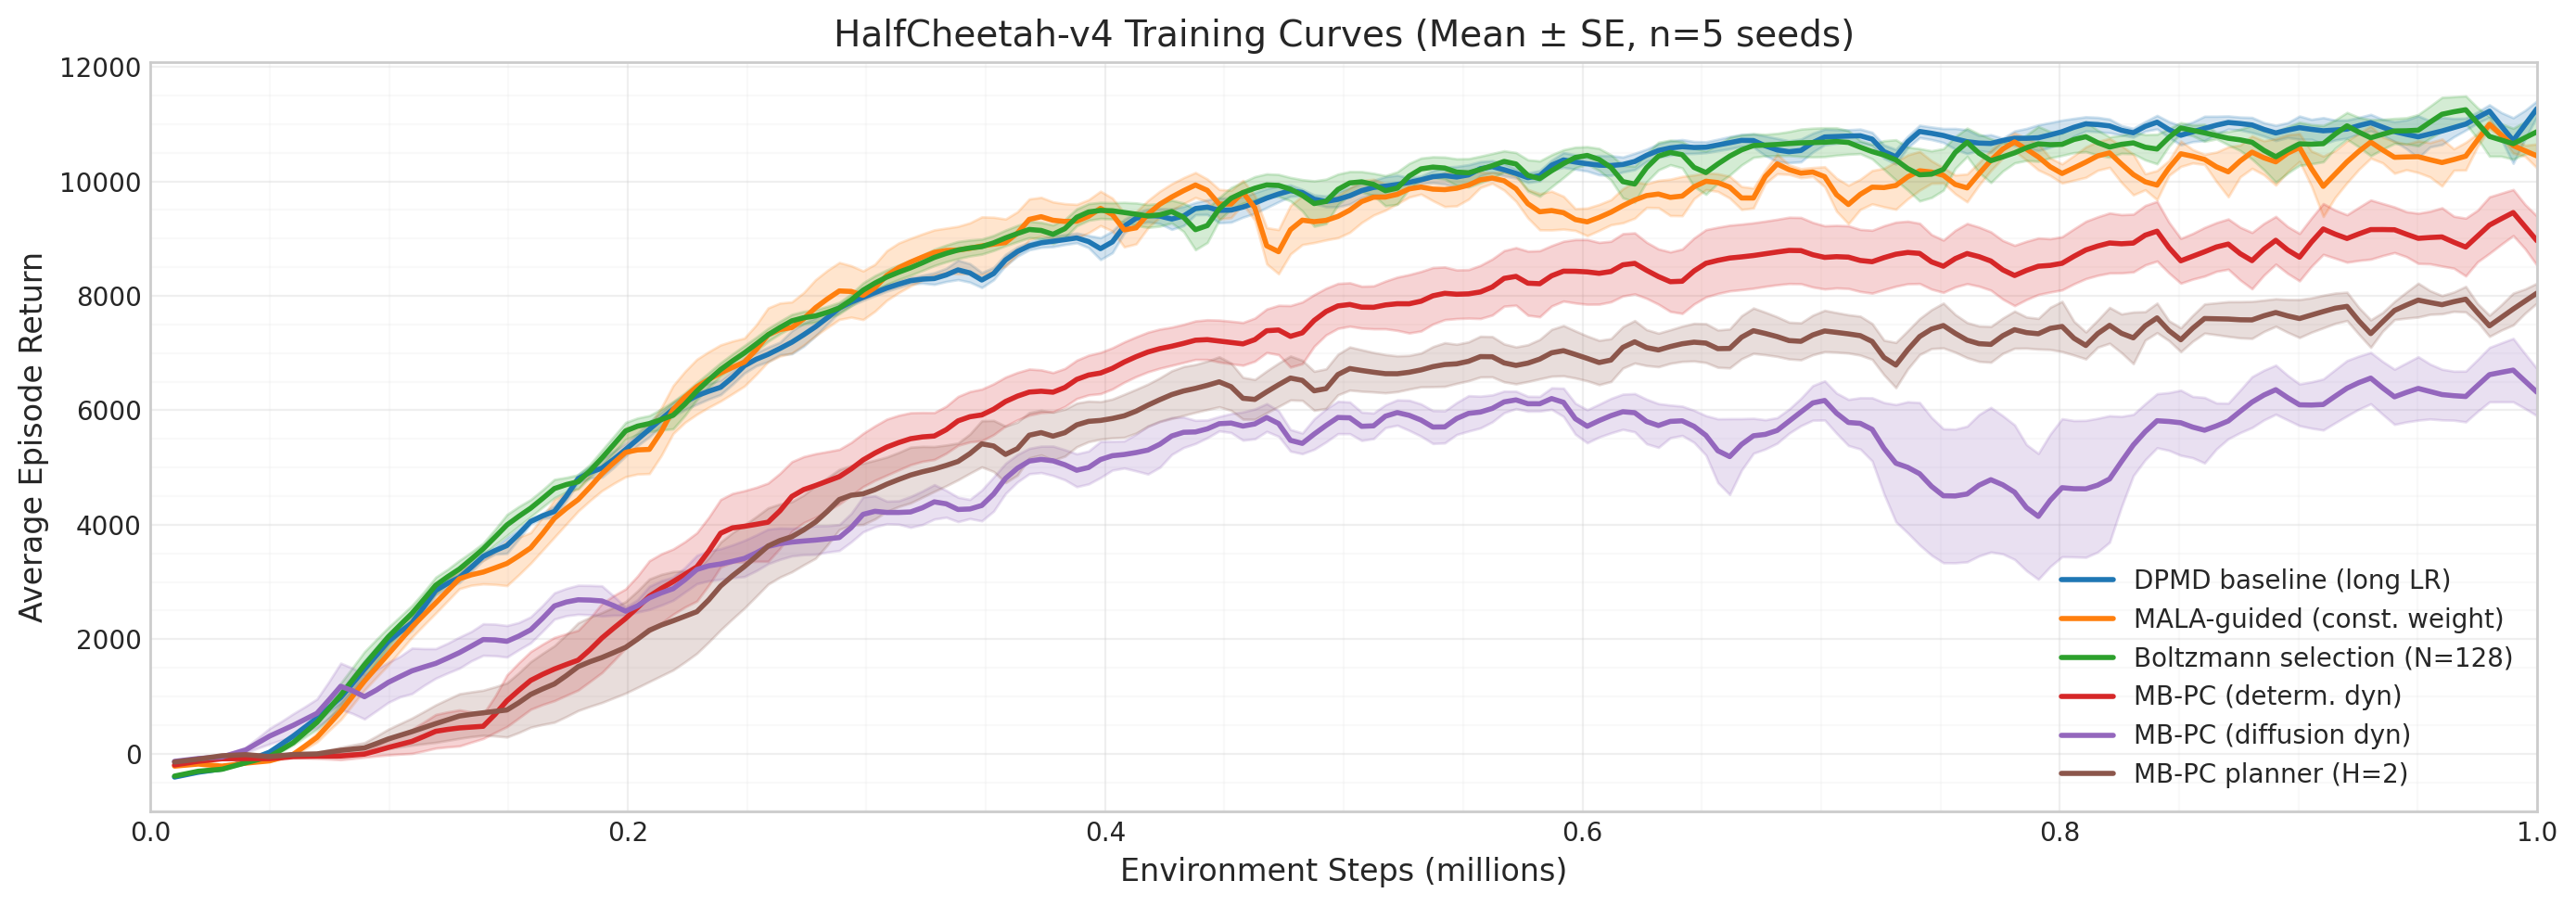
\includegraphics[width=\textwidth]{training_curves.png}
  \caption{Training curves on HalfCheetah-v4 showing mean episode return $\pm$ standard error across 5 seeds. The DPMD baseline achieves the highest final return but uses learning-rate annealing, which is incompatible with continual learning (see \cref{sec:lr-caveat}). Among constant-LR methods, Boltzmann selection and MALA-guided DPMD perform best. Model-based methods with deterministic dynamics reach roughly $9000$ return, while diffusion dynamics and short-horizon planning underperform.}
  \label{fig:training-curves}
\end{figure*}

\subsection{Inference-time methods and the constant-weight anomaly}

We first evaluate the inference-time methods that use $Q$ only at sampling time, not in the training loss.

\paragraph{Constant-weight diffusion + Boltzmann selection.}
The simplest method in our progression---training the diffusion policy by pure behavior cloning and performing many-particle Boltzmann selection at inference time---achieves $10866$ return (SE $\approx 370$) using $N=128$ particles and selection temperature $\lambda_{\text{sel}}=64$.
Since this variant does not use $Q$ in the diffusion loss and consults it only through the selection distribution, it provides a strong baseline for inference-time scaling: decision-time compute grows linearly with $N$ and can be adjusted without retraining.
This is the strongest constant-LR method in our comparison.

\paragraph{MALA-guided sampling.}
Adding gradient-based MALA corrections on top of constant-weight training achieves $10443$ average return (SE $\approx 209$) over five seeds.
This configuration uses a single action particle with guidance strength $\lambda=16$ and two MALA steps per diffusion level.
As shown in \cref{fig:training-curves}, the learning curves exhibit similar stability to the baseline throughout training.
As of now, MALA guidance slightly underperforms pure Boltzmann selection in this setting, though it is much simpler, using only a single action particle, constant learning rates, and no artificial action noise injection.


\subsection{Model-based compositional guidance and planning}

We next evaluate model-based compositional guidance, which replaces the monolithic $Q$-function with a compositional objective $J(s,a) = \mathbb{E}[r(s,a,s') + \gamma V(s')]$.
These methods represent the more complex end of our progression, and our results show that this additional complexity does not yet translate to improved performance.
However, we demonstrate that all configurations can be trained stably online from scratch---an important proof of concept.

\paragraph{Deterministic dynamics ($H=1$).}
With a deterministic dynamics model (trained by MSE regression) and one-step lookahead, our best configuration reaches $8963$ average return (SE $\approx 430$).
Despite being below the best $Q$-based methods, this result demonstrates that a compositional objective can support stable online learning when dynamics are relatively easy to model.
The gap to the $Q$-based methods suggests that either the learned $V_\xi$ is not as well-calibrated as $Q_{\min}$, or that errors in the dynamics model introduce noise into the guidance signal.

\paragraph{Diffusion dynamics.}
Replacing the deterministic dynamics with a diffusion-based dynamics model yields $6316$ return (SE $\approx 413$).
We attribute this drop partly to the increased variance induced by stochastic dynamics inside the planner and partly to the difficulty of accurately modeling the one-step transition distribution with a diffusion model.
Notably, this is the first time (to our knowledge) that a diffusion policy and a diffusion dynamics model have been jointly trained online from scratch in a continuous-control RL setting.

\paragraph{Short-horizon planner ($H=2$).}
Extending to two-step planning by chaining together one-step policies with a deterministic dynamics model achieves $8046$ return (SE $\approx 173$).
This is slightly below the $H=1$ configuration ($8963$), suggesting that the additional complexity of planning over action sequences does not yet pay off in this setting---compounding model error appears to outweigh the benefit of reduced dependence on the value function.


\section{Discussion and Limitations}
\label{sec:discussion}

The experiments highlight both the promise and the challenges of inference-time and compositional guidance for diffusion policies.
Our progression of methods---from simple Boltzmann selection through MALA guidance to full model-based compositional planning---reveals a consistent pattern: the simpler methods currently outperform the more complex ones.
This is the opposite of what we would ideally like to see, but we are optimistic that the more complex methods already perform stably and that the design space around them is large. We have only scratched the surface so far in investigating what these algorithms are most sensitive to.
We organize our discussion around four themes.

\subsection{Inference-time guidance suffices}

Our constant-weight variants rely on $Q$ only at inference time, either through MALA or Boltzmann selection, and achieve performance close to the LR-annealed DPMD baseline while using constant learning rates suitable for continual learning.
In contrast, disabling inference-time selection while keeping $Q$-weighted score matching led to a sharp drop in performance.
Together with the effective-sample-size control used in DPMD---which intentionally keeps the normalized weights close to uniform for stability---this suggests that the mirror-descent tilt plays a smaller practical role than one might expect: for much of training the reweighted loss is numerically close to an unweighted denoising objective, and attempts to let the weights vary more aggressively tend to interact poorly with noisy Q-estimates.

From this perspective, a simple and robust recipe emerges: fit the diffusion policy with uniform weights, then apply the critic only at decision time.
This stands in contrast to the original DPMD emphasis on training-time reweighting and suggests that, at least in our regime, inference-time tilting and filtering are the more reliable tools.
Importantly, this recipe is also more compatible with continual learning settings where the training horizon is not fixed in advance.

\subsection{Guidance strength, temperatures, and filtering vs gradients}

Performance was highly sensitive to how $Q$ was normalized and to the effective ``temperature'' with which it was injected.
Different algorithms required widely different optimal guidance strengths.

This sensitivity can be understood by noting that $\lambda$ interacts differently with the critic in each setting.
In MALA, $\lambda$ multiplies gradients in energy space; too small and guidance is ineffective, too large and the chain takes unstable steps that move samples off-manifold or cause low acceptance rates.
In Boltzmann selection, $\lambda_{\text{sel}}$ appears inside the softmax over Q-values; larger values sharpen the distribution over already-valid samples and do not threaten stability.

More broadly, we observed that sampling 128 actions and selecting via Boltzmann weighting matched or slightly exceeded the performance of gradient-based MALA guidance.
This suggests that, in this environment, much of inference-time ``planning'' reduces to \emph{filtering}: the diffusion prior already places substantial mass near good actions, and the critic's primary role is to rank them rather than to produce a globally accurate gradient field. However, we expect the importance of gradient to increase when action spaces become higher dimensional or when planning over a longer horizon.



\subsection{Limitations and future work}

Our study has several limitations.
First, we evaluate only on HalfCheetah-v4; other environments, especially those with sparser rewards or more challenging dynamics, may show different trade-offs between guidance mechanisms.
Second, due to compute constraints we did not perform exhaustive hyperparameter sweeps over guidance strengths, numbers of MALA steps, numbers of particles, or planning horizon.
The reported numbers should be interpreted as specific design points rather than definitive optima.
Third, the model-based planner is sensitive to learning-rate scales, guidance temperatures, and particle-refresh settings, and we did not systematically ablate each design choice.

Promising directions for future work include:
(i) Training the value function in our compositional objective on-policy, similar to how Q is trained.
(ii) Expressing a multi-step policy as the composition of one-step policies and a dynamics model and applying inference-time guidance in a more principled way.
(iii) Investigating how performance of guided vs filtered methods depend on the dimension of the action space and planning horizon.


\section*{Acknowledgements}

This work builds directly on the publicly released DPMD codebase of \citet{ma2025soft}, and I thank the authors for providing a high-quality implementation.
Code for all experiments is available at \url{https://github.com/pnielsen2/inference_mirror_descent}.

This is a work in progress.
Comments, suggestions, and collaboration inquiries are welcome---please contact the author at the email address above.

\section*{Impact Statement}

This work studies diffusion-based reinforcement learning algorithms in simulated continuous-control benchmarks.
Its primary impact is methodological: to clarify how inference-time guidance and compositional objectives can be used to improve diffusion policies.
We do not foresee immediate societal risks beyond those already associated with progress in general-purpose RL and generative modeling.
Any real-world deployment of such methods in safety-critical domains would require additional safeguards, domain-specific constraints, and human oversight.

\bibliography{refs}
\bibliographystyle{icml2026}

\end{document}
